\documentclass[12pt]{article}
%\usepackage{report}

\usepackage[utf8]{inputenc} % allow utf-8 input
%\usepackage[T1]{fontenc}    % use 8-bit T1 fonts
\usepackage[colorlinks=true, linkcolor=blue, citecolor=blue, urlcolor=blue]{hyperref}       % hyperlinks
\usepackage{url}            % simple URL typesetting
\usepackage{booktabs}       % professional-quality tables
\usepackage{amsfonts}       % blackboard math symbols
\usepackage{nicefrac}       % compact symbols for 1/2, etc.
%\usepackage{microtype}      % microtypography
\usepackage{lipsum}		% Can be removed after putting your text content
\usepackage{graphicx}
\usepackage{footnote}
\usepackage{doi}
\usepackage{comment}
\usepackage{multirow}
\usepackage{textcomp}
\usepackage{gensymb}
\usepackage{float}
\usepackage{amsmath}
%\usepackage{subfigure}
\usepackage{subcaption}
\usepackage{setspace}
\usepackage[skip=10pt plus1pt]{parskip} %I got rid of indent=30pt to make the paragraphs line up nicer - GI
\usepackage[top=1.5in, bottom=1.5in, left=1in, right=1in]{geometry}
\usepackage{titlesec}
\begin{document}


%%%%%%%%%%%%%%%%%%%%%%%%%%%%%%%%%%%%%%%%%%%%%%%%%%%%%%%%%%%%%%%%%%%%%%%%%%%%%
%%%                                                                      %%%
%%%                  ������  !!!  READ ME  !!!  ������                   %%%
%%%                                                                      %%%
%%%    note with your intials if any changes/comments are added! thx     %%%
%%%                                                                      %%%
%%%%%%%%%%%%%%%%%%%%%%%%%%%%%%%%%%%%%%%%%%%%%%%%%%%%%%%%%%%%%%%%%%%%%%%%%%%%%


\begin{titlepage}
    \centering
    
\includegraphics[width=3cm]{Figures/crest.jpg}\par
    \vspace{0.3cm}
    {\scshape\Large School of Mathematical Sciences \par}
    \vspace{0.25cm}
    {\scshape\Large The University of Southampton \par}
    \vspace{0.25cm}
    {\Large MATH 6149 - Modelling with Differential Equations \par}
    \vspace{0.5cm}
    {\huge\bfseries On the equations of motion of a swing\par}
    \vspace{0.5cm}
    {\Large Ben Crossland \par}
    \vspace{0.25cm}
    {\Large Chin Phin Ong (Linus) \par}
    \vspace{0.25cm}
    {\Large Gabriella Iuliano\par} %I dont know your full name, please insert full name here -L
    \vspace{0.25cm}
    {\Large Jacob Smith \par}
    \vspace{0.25cm}
    {\Large Zayn Khan \par}
    %\vspace{0.25cm}
    {\large  \par}
    \vfill
    {\large January 2025 \par}
\end{titlepage}

\begin{abstract}
    %insert abstract here -L 
    We model the motion of a kiiking swing by approximating a pendulum to find the optimal technique for the rider.  By periodically standing and squatting, the centre of mass of our system shifts towards and away from the origin.  We explore how to mathematically describe the dynamics of our system and determine the number of swings necessary for the kiiker to make a full rotation on the swing.
\end{abstract}

\section{Introduction}
The aim of this coursework is to investigate the behaviour of a person standing on a swing and moving the swing via an up and down motion of the body on the swing, like in the extreme sport kiiking.

Kiiking (from the Estonian word `kiik', meaning swing) is a sport where the goal is to make a full rotation of the swing (that is attached to the fulcrum via steel beams). The person who successfully does a full rotation with the longest shaft is the winner. The way one would operate a kiiking swing is by `pumping', standing up and squatting down on the swing. The act of standing on the swing creates a constructive force. With the correct technique, one will be able to swing higher and higher, and finally do a full rotation.

In the following sections, we will attempt to model a person on a kiiking swing using differential equations to find the optimal kiiking pattern, solve the differential equation numerically, and discuss the limitations of the model. We found that despite making quite a lot of assumptions about our swing, these assumptions did not stop us from being able to model the swing realistically. %-L

\section{On Swings}
%Multiple studies have been conducted on the optimal swing pattern. \cite{wirkus1998pump, klimina2022optimal, Yan2005swing}
%can write up about what steps were taken (like going to an actual swing set) to effectively express the model in equation form) -L

%maybe this section can be combined with the section below (on the model) - thoughts? -L

% i think actually we should leave this separate somewhat, and maybe include more on assumptions made (e.g no friction or dissaptivie terms, point mass etc) for now? But maybe see how we get on and then maybe we can make these into subsections idk - JS

%I feel like maybe it can be a subsection in the next section as an introduction to the problem? -GI
In order to begin our model, we must state some of the assumptions that we made.  We assume that the kiiker, swing and connecting rods form a point mass located at their center of gravity, hence, ignoring air resistence.

We can model our swing as a pendulum with variable length $r$.  We can model our rider with point mass $m$ and $r$ is the distance between the rider's centre of mass and the swing's support $O$ \cite{wirkus1998pump}.  

When the rider stands up the rider's centre of mass moves closer to the origin ($r = r_{min}$)and when the rider squats down, the centre of mass moves further away from the origin ($r = r_{max}$). As the rider constantly moves from standing up to squatting down, the distance from the point of support to the centre of mass consists of a constant plus a periodically changing length \cite{William1996standing}, effectively creating a variation in the pendulum length. This `pumping' motion is what kiikers use to swing higher and higher. 

\section{The Model}
\subsection{Newton's laws in polar coordinates}
%derivation of the differential equation, and solving, parameter space... -L

To model the swings accurately we use Newton's second law %should we add ref? -JS
of motion in polar coordinates. We can write the position of the swing, $\mathbf{r} (t)$ 
%can someone double check should this be bold? -js
as it's vector components and the basis vector $\mathbf{e_r}$,
$$\mathbf{r}(t) = r(t)\mathbf{e_r},$$
and we can describe the change in basis vectors for polar coordinates from the Cartesian basis (and vice versa) as (see figure \ref{figBasis}) the following:
\begin{align}
    \mathbf{e_r} &= \cos(\theta) \mathbf{e_x} + \sin(\theta) \mathbf{e_y}, \\
    \mathbf{e_\theta} &= -\sin(\theta) \mathbf{e_x} + \cos(\theta) \mathbf{e_y},\\
    \mathbf{e_x} &= \cos(\theta)\mathbf{e_r} - \sin(\theta) \mathbf{e_\theta},\\
    \mathbf{e_y} &= \sin(\theta) \mathbf{e_r} + \cos(\theta) \mathbf{e_\theta}.
\end{align}

\begin{figure}[ht]
    \centering
    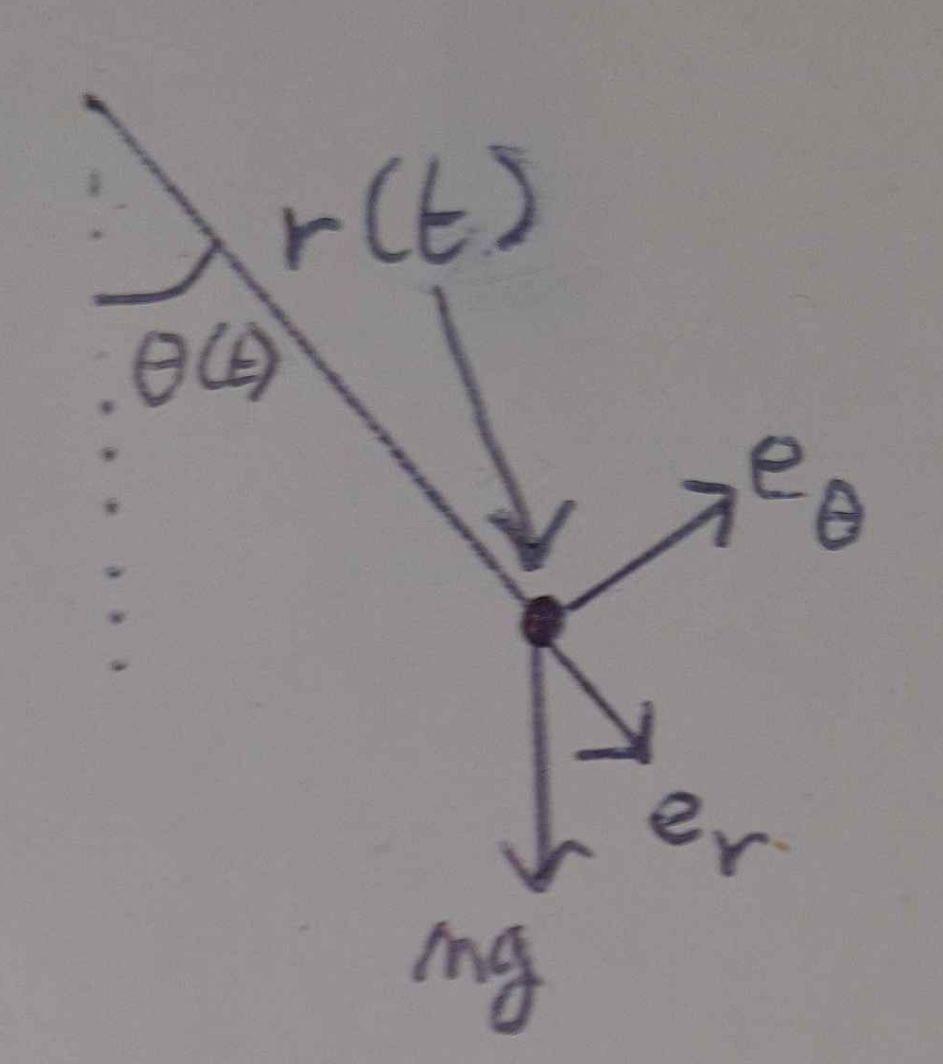
\includegraphics[width=0.3\textwidth]{Figures/Swing.png}
    \caption{The position $r(t)$ of the swing at time $t$. $\theta(t)$ describes the angle that the swing makes with a vertical axis. $\mathbf{e_r}$ and $\mathbf{e_\theta}$ are the respective basis vectors and $mg$ is the total weight on the swing. \label{figBasis}} %fixed basis vectors and clarified mg to total weight, not the swing.
\end{figure}
Using the usual dot notation to indicate a derivative with respect to time, we can also find that (see Appendix A.1 on Newton's Laws):
\begin{align}
    \dot{\mathbf{e_r}} &=  \dot{\theta}\mathbf{e_\theta},\\
    \dot{\mathbf{e_\theta}} &= -\dot{\theta} \mathbf{e_r}
\end{align}
Newton's second law gives us that $\mathbf{F} = m\mathbf{a}$, where $\mathbf{F}$ is the net force, $m$ is the mass, and $\mathbf{a}$ is the acceleration. In the case of our swing we therefore have that:
$$\mathbf{F} = mg \mathbf{e_x} - T \mathbf{e_r}.$$
Here, $m$ is the mass of the swing, $g$ is the acceleration due to gravity, and $T$ is the tension of the rope that attaches the swing to a fixed point. We can find the acceleration of the swing by taking two derivatives of it's position (see Appendix A.2 on Newton's Laws),
$$
    a = (\ddot{r} - r \dot{\theta}^2) \mathbf{e_r} + (2\dot{r} \dot{\theta} + r \ddot{\theta}) \mathbf{e_\theta}.
$$
If we rewrite the $\mathbf{e_x}$ in $F$ in terms of $\mathbf{e_r}$ and $\mathbf{e_\theta}$, we then get that Newton's second law gives us:
$$mg(\cos(\theta) \mathbf{e_r} - \sin(\theta) \mathbf{e_\theta}) - T\mathbf{e_r} = [(\ddot{r} - r \dot{\theta}^2) \mathbf{e_r} + (2\dot{r} \dot{\theta} + r \ddot{\theta}) \mathbf{e_\theta}]m$$

Looking at the $\mathbf{e_r}$ and $\mathbf{e_\theta}$ components separately gives us two equations:
\begin{align}
    \ddot{r} - r \dot{\theta}^2 &= g\cos(\theta) - \frac{T}{m},\label{ODE1}\\
    2\dot{r} \dot{\theta} + r \ddot{\theta} &= -g\sin(\theta).\label{ODE2}
\end{align}
Note that the $r \dot{\theta}^2$ term is the centrifugal force and the $2 \dot{r}\dot{\theta}$ corresponds to a Coriolis term.  Solving the two coupled ordinary differential equations will allow us to describe the motion more accurately.

Looking at equation \ref{ODE2}, and multiplying both sides of the equation by $r$ allows us to rewrite equation \ref{ODE2} as:
\begin{equation}
    \frac{d}{dt}(r^2 \dot{\theta}) = -gr\sin(\theta)
    \label{ODE3}
\end{equation}
We can then integrate both sides of the equation about a small interval $-\epsilon$ to $\epsilon$ and take the limit as $\epsilon \to 0$, where we let $\dot{\theta}$ be either $>0$ or $<0$ in the small step in the interval (it does not change sign) and choose $\epsilon$ to be $\ll 1$. This gives that the $RHS = 0$ as the $RHS$ is continuous in $t$ and we are integrating over a small discontinuity (see figure \ref{Figrdiscont} and \ref{Figrjump}),
\begin{figure}[H]
    \centering
    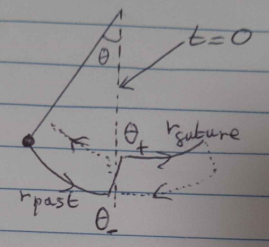
\includegraphics[width=0.3\textwidth]{Figures/rdiscont.png}
    \caption{A small interval $- \epsilon$ to $\epsilon$ about a discontinuity at $t=0$ and the assumption that $\dot{\theta} >0$ in the interval, allows us to label $r(t)$, the length from the centre of the swing and $\theta$, the angle of the swing from a $y$ axis of the two sides as $r(t) = r_{past}$ and $\theta = \theta_-$ before $t=0$ and $r(t) = r_{future}$ and $\theta = \theta_+$ after $t=0$. The solid line represents swinging anticlockwise and the dotted line is anticlockwise.\label{Figrdiscont}}
    \label{fig1}
\end{figure}

\begin{figure}[H]
    \centering
    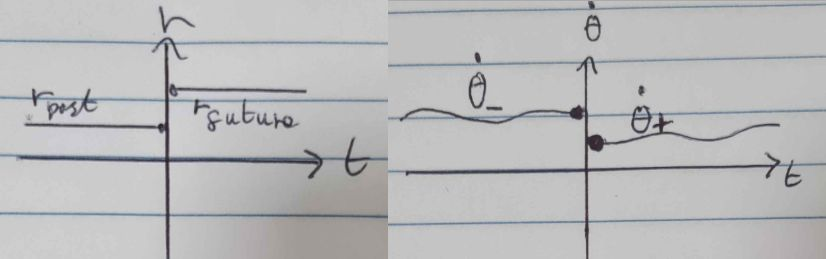
\includegraphics[width=0.7\textwidth]{Figures/Jumpdiscont.jpg}
    \caption{On the left, $r$ goes from some constant value $r_{past}$  for $t = -\epsilon$ to $r_{future}$ for $t=\epsilon$. Similarly, $\dot{\theta}$ is some value $\dot{\theta}_-$ just before $t=0$ and goes to $\dot{\theta}_+$ immediately after the discontinuity. \label{Figrjump}}
    \label{fig1}
\end{figure}
% I DONT REMEMBER WHY, WE NEED TO ASK
we are left with,
$$\lim_{\epsilon \to 0} \int_{-\epsilon} ^ \epsilon \frac{d}{dt}(r^2 \dot{\theta}) = 0.$$
Which implies that:
\begin{equation}
\lim_{\epsilon \to 0}\big[r^2 \dot{\theta}\big]^\epsilon_{-\epsilon} = 0,\label{Thetaeq}
\end{equation}
and therefore we can find the relationship between $\dot{\theta_-}$ and $\dot{\theta}_+$, the $\dot{\theta}$ evaluated at $t=-\epsilon$ and $t = \epsilon$ respectively. Equation \ref{Thetaeq} implies:
$$\lim_{\epsilon \to 0}(r^2_{past} \dot{\theta} \big|_{t= -\epsilon} - r^2_{future} \dot{\theta} \big|_{t=\epsilon}) = 0$$

and so,
\begin{align}
    r^2_{past} \dot{\theta}_- - r^2_{future} \dot{\theta}_+ &= 0 \\
    \implies \dot{\theta}_+ &= \frac{r^2_{past}}{r^2_{future}}\dot{\theta}_-. \label{eq: ratio of past and present velocity}
\end{align}
%i dont like my explanation here-JS

% i wasnt really sure what to write for our assumptions for why we put the heaviside in - JS

%-JS
\subsection{A Recursive Solution}
From here, it's useful to recall that $\theta_-$ and $\theta_+$ are separated in time as this is what we took the integral over. More specifically, we took the integral over the discontinuous part of our function, that being those moments in which the kiiker stands up straight or squats back down. Therefore, we can interpret equation \ref{eq: ratio of past and present velocity} as the relationship between the angular velocity of the swing immediately before the change in radius and the angular velocity of the swing immediately after the change in radius. The rest of the motion is well described by the continuous parts of our equation. As such, our model describes the entire motion of the swing by piecing together an $N$ number of differential equations that are identical aside from their initial conditions which are determined by equation \ref{eq: ratio of past and present velocity}. We will hence label the multiplier of velocity  when the kiiker stands up as $a$ and the multiplier of velocity when the kiiker squats down as $a^{-1}$ like so: 

\begin{align}
    \dot{\theta}_+ &= a^2 \,\dot{\theta}_- \,\, \text{when standing up} \\
    \dot{\theta}_+ &= a^{-2} \,\dot{\theta}_- \,\,\text{when squatting down }\\
\end{align}
where $a = \frac{r_{max}}{r_{min}}$ as is implied by equation \ref{eq: ratio of past and present velocity}.\\

With this in mind, an optimal method of swinging becomes apparent as we can observe that $a >1$ and hence standing results in increasing one's speed and sitting down results in decreasing one's speed, both in proportion to the speed that the kiiker is already going. However, one must squat down in order to stand back up again, so we must try and maximise speed when the kiiker stands up and minimise it when they squat down. Hence, the kiiker should stand up when $\theta = 0$ (when the angular velocity is at its maximum) and squat back down when $\theta$ is at its maximum (when the angular velocity is 0 ) for that swing. With this method, velocity does not change when squatting down and only changes at $\theta = 0$ so this is the only discontinuous point in terms of angular velocity. We will later break our discontinuous equation of motion up into continuous pieces indexed by $n$ and our previous rationale has allowed us to provide initial conditions for every other piece:
\begin{equation}
    \dot{\theta}_{2m} = (-1)^ma^{2m}\dot{\theta}_0, \, m \in \mathbb{Z}.
\end{equation}
In this way, $m$ can be interpreted as the number of swings, where $\dot{\theta}_0$ is the small velocity that the swing starts with due to perturbations. The following figure demonstrates this in terms of the phase space in figure \ref{fig:phase_space}. The phase space was obtained by numerically solving the differential equation in pieces, as we have the relationship between $\dot\theta_{+}$ and $\dot\theta_{-}$ for any number of swings $n$. It is obvious that $(\dot\theta_{+})_n = (\dot\theta_-)_{n+1}$, so we can obtain initial values for the numerical solution. The plot of $\theta$ against $t$ plot is also easily obtained and is shown in Fig. \ref{fig:theta_time}.
\begin{figure*}[ht]
    \centering
    \begin{subfigure}[b]{0.49\textwidth}
        \centering
        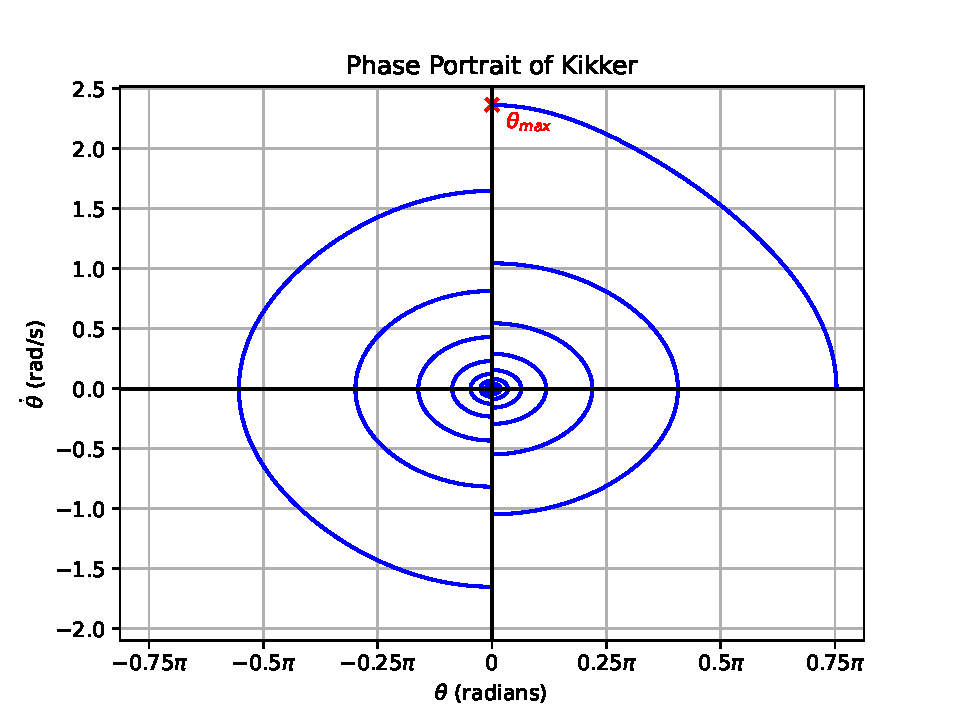
\includegraphics[width=\textwidth]{Figures/phase_plot.pdf}
        \caption{Phase space of the swing, ($\theta$,$\dot{\theta}$), parametrised by $t$.}
        \label{fig:phase_space}
    \end{subfigure}
    \hfill
    \begin{subfigure}[b]{0.49\textwidth}
        \centering
        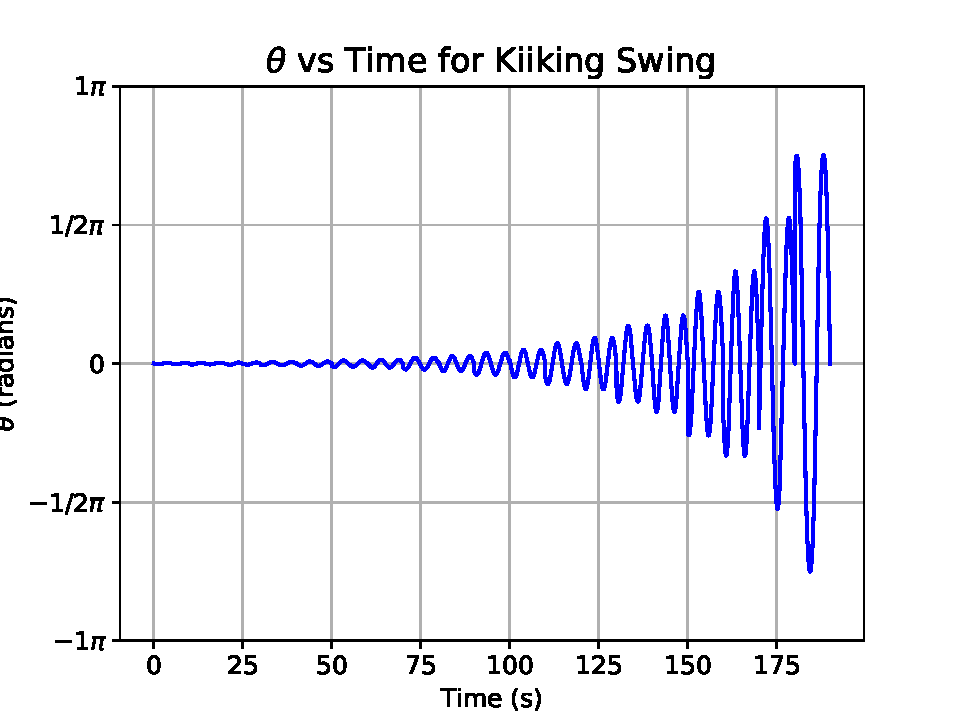
\includegraphics[width=\textwidth]{Figures/thetatimeplot.pdf}
        \caption{Theta against time}
        \label{fig:theta_time}
    \end{subfigure}
    \caption{Plots of the differential equation Eqn. \ref{ODE3}, taking into account the discontinuities. Obtained via numerical solution.}
\end{figure*}
If we need only to determine the number of swings a kiiker requires to go all the way around then this can be found as a corollary of what we've already done. We can easily work out the angular velocity required at $\theta = 0$ (the bottom of the swing) to reach the top (and therefore go all the way around) using energy by equating gravitational and kinetic energy. Taking the pivot of the swing to be the zero point, where above the swing the distance will be positive and below the swing it will be negative:
%clarification of the physics above, and fixed typo in equationbelow. please correct me if anything is off -L
\begin{align}
    2mgr = \frac{1}{2}mv^2 \,\, \text{where $v$ is velocity }\\
    \implies v = \pm 2\sqrt{gl} \,\, \text{where $l$ is length of the swing}
\end{align}

As we are working in radians, the distance around the circle is $\theta l$ so we therefore have $v = \dot{\theta}r$ implying that $|{\dot{\theta}_{2m}}| >  \frac{2\sqrt{gl}}{l}$ must be satisfied at $\theta = 0$ in order to complete a rotation on that swing.

Therefore, by substituting our previous equation for $|{\dot{\theta}_{2m}}|$ at $\theta = 0$, we find that the final swing is the first integer that satisfies:
\begin{equation}
    m >\frac{\ln\left({2 \sqrt{g}}\right) - \ln{\left(\dot{\theta}_0 \sqrt{l}\right)}}{2\ln{a}}.
\end{equation}

%-ZK
\subsection{Motion in between discontinuities}
We still need to model the motion for areas where the Kiiker is staying at the same height (i.e. in between the discontinuities of the Kiiker changing their height by squatting or standing). We begin by by taking $r$ to be a constant. This transforms equations \ref{ODE1} and \ref{ODE2} into:
\begin{align}
    \dot{\theta}^2 &= -\frac{g}{r} \cos{\theta} + \frac{T}{mr} \label{ODE1 const r}
    \\\ddot{\theta} &= -\frac{g}{r}\sin{\theta} \label{ODE2 const r}
\end{align}

Multiplying equation \ref{ODE2 const r} by $\dot{\theta}$, we can combine and recast equations \ref{ODE1 const r} and equation \ref{ODE2 const r} as:
\begin{align}
    \dot{\theta}^2 = -\frac{g}{r}\cos(\theta) + \frac{T}{mr}
\end{align}

In terms of derivatives:
\begin{align}
    \frac{d}{dt}(\frac{1}{2}\dot{\theta}^2) + \frac{d}{dt}(-\frac{g}{r}\cos(\theta)) &= 0
    \implies \frac{d}{dt}(\frac{1}{2}\dot{\theta}^2 - \frac{g}{r}\cos(\theta)) = 0 \label{combined derivative eqn}
\end{align}

Integrating equation \ref{combined derivative eqn} with respect to time we obtain:
\begin{align}
    \frac{1}{2}\dot{\theta}^2 &- \frac{g}{r}\cos(\theta) = c \label{integrated derivative eqn}\text{,  where $c$ is a constant.}
    \\&\implies{\cos{\theta} = \frac{r}{g}(\frac{1}{2}\dot{\theta}^2 - c)}
\end{align}

Plugging this into equation \ref{ODE1 const r}:
\begin{align}
    \dot{\theta}^2 &= -\frac{g}{r} \frac{r}{g}(\frac{1}{2}\dot{\theta}^2 - c) + \frac{T}{mr}
    \\&\implies \frac{T}{mr} = \frac{3}{2}\dot{\theta}^2 - c
\end{align}

Rearranging for $T$, we arrive at:
\begin{align}
    \frac{T}{mr} &= \frac{3}{2}\dot{\theta}^2 - c
    \label{tension eqn}
\end{align}

As stated, the larger model is pieced together from the smaller continuous equations of the motion for the swing given above.
After each discontinuity, the equations above apply to the swing with different initial conditions.
Generally, the continuous motion of the swing is described by \ref{integrated derivative eqn}:
\begin{align}
    \frac{1}{2}\dot{\theta}^2_n - \frac{g}{r}\cos{\theta_n}&= c_n,
    \label{coninuous motion eqn}
\end{align}
where $n$ is the number of discontinuities the kiiker has passed through (i.e. the number of times they have stood or squatted).

After each discontinuity where the kiiker stands at the lowest point of the swing our angular velocity changes (so every other ODE starting at $\dot{\theta}_0$), following the equation:
\begin{align}
    \dot{\theta}_{2m} &= (-1)^{m} a^{2m}\sigma,
    \label{discontinuity reln}
    \text{ where $a = \frac{r_{max}}{r_{min}}$ and $\sigma = \dot{\theta}_0$ (the initial angular velocity) at } \theta_{2m} = 0.
\end{align}

% We only have this for every other equation but we can  use theta dot = 0 when t = 0 on other equations. So we'll get two different expressions for c_n. - BC
Combining this with \ref{coninuous motion eqn} in cases where $\theta = 0$ we have:
\begin{align}
    \frac{1}{2}(-1)^{m}a^{4m}\sigma^2 - \frac{g}{r} = c_{2m}
\end{align}

Now that we have an expression for $c_n$ we return to \ref{tension eqn}:
\begin{align}
    \frac{T_{2m}}{mr} = \frac{3}{2}\dot{\theta}_{2m}^2 - \frac{1}{2}(-1)^{m}a^{4m}\sigma^2 + \frac{g}{r}
\end{align}
%should put theta dot_n here to keep indexing consistent. - BC
This transforms \ref{ODE1 const r} from its original form, to:
\begin{align}
    \dot{\theta}_{2m}^2 = -\frac{g}{r}\cos{\theta_{2m}} + \frac{3}{2}\dot{\theta}_{2m}^2 - \frac{1}{2}(-1)^{m}a^{4m}\sigma^2 + \frac{g}{r}
    \\\implies\dot{\theta}_{2m}^2 = 2\frac{g}{r}(\cos{\theta}_{2m}-1) +a^{4m}\sigma^2 
    \label{odd final theta dot eqn}
\end{align}

For $\theta$, we would take the square-root of \ref{odd final theta dot eqn}. The positive solution would apply when the kiiker swings forward, while the negative solution would apply when they swing backwards.

For cases where the kiiker squats as the swing reaches its highest point, we have $\dot{\theta}_{2m-1} = 0$ at some $\theta_{2m-1,max}$ (the value of $\theta$ at the point the swing reaches its maximum amplitude), transforming \ref{coninuous motion eqn} into:
\begin{align}
    -\frac{g}{r}\cos{\theta_{2m-1,max}} = c_{2m-1}
    \\&\implies \frac{T_{2m-1}}{mr} = \frac{3}{2}\dot{\theta}_{2m-1}^2 + \frac{g}{r}\cos{\theta_{2m-1,max}}
    \\&\implies \dot{\theta}_{2m-1}^2 = \frac{2g}{r}(\cos{\theta_{2m-1}}-\cos{\theta_{2m-1,max}})
    \label{even final theta dot eqn}
\end{align}

Where the positive solution for $\dot{\theta}$ applies where the swing is at the maximum swinging forward, and the negative solution applies where the swing is at the maximum swinging backwards.

Assuming the kiiker begins at $\theta_0 = 0$ with some small $\dot{\theta} \neq 0$, we take odd values of $n$ when the swing is at a maximum where \ref{even final theta dot eqn} applies, and even values of $n$ when the swing passes through the centre point, where \ref{odd final theta dot eqn} applies.

\section{Limitations of the Model}
%limitations - e.g. valid for certain angles, works for solid steel swing pole, etc. -L

Our model is based on the following assumptions.
Firstly, the kiiker and swing form a point mass located at the centre of gravity between the two. For this reason, we may neglect air resistance. In reality, there would be some resistive forces, but as the kiiker is actively increasing their amplitude we have ignored damping effects that are overcome anyway.
Secondly, we assume the swing only moves in the plane of motion - our model does not recognise transverse motion that is not in the plane of the swinging. For a system constructed from metal poles rather than chain, this is reasonable assumption, as the poles are rigid and will not drift sideways to any meaningful degree. The poles also allow us to assume they do not compress or extend throughout the motion, so changes in $r$ only come from the kiiker. Furthermore, we assume the poles move smoothly around the frame with no frictional effects, which can be realistically acheived with the use of a lubricant. We have also ignored the very negligible changes in force due to gravity as the kiiker and swing move up and down.

Our equations also ignore the time taken for the kiiker to squat and stand, it is assumed that the motion of the centre of gravity between $r_{max}$ and $r_{min}$ is immediate. In reality, the kiiker would spend some fraction of time standing, but this period of time is very small compared to the period of a swing, so has been modelled as a discontinuity in length $r$.
Our equations also stop accurately modelling the system once the kiiker has built up the energy to finally go all the way around the frame. Physically, this happens when the kiiker reaches the lowest point in their motion before swinging up and around.

\section{Conclusion}
In conclusion, we successfully modeled the motion of a kiiking swing under the air resistance is negligible, and the rod maintains a constant length. By formulating Newton’s second law in polar coordinates and analyzing the change in basis vectors, we derived an equation for the acceleration of the swing. Separating the equations for \(\mathbf{e_r}\) and \(e_{\theta}\), we solved the coupled ordinary differential equations, enabling us to interpret the relationship between the angular velocity of the swing immediately after a change in radius.  

Additionally, we determined the optimal swinging technique by deriving the equation for \(\dot{\theta}_{+}\) during standing and squatting. Our results indicate that to maximize the amplitude of the swing, the rider should stand up when \(\theta = 0\) and squat back down when \(\theta\) reaches its maximum. We visualized this behavior by plotting the phase portrait of the kiiker and a graph of \(\theta\) versus time (as shown in Figure 4). Furthermore, we identified the maximum velocity of the swing before the solution closes, corresponding to the moment when the rider completes a full rotation.  

Finally, we extended our model to describe the motion in regions where the kiiker maintains a constant height between discontinuities.  

However, our model is based on several simplifying assumptions, such as neglecting air resistance and assuming instantaneous transitions between standing and squatting. In reality, these factors play a role in the dynamics of the swing.  Hence, for future models, we should see how getting rid of these assumptions would affect the model that we made.

%conclusion, futher improvement suggestions - if improvements can be implemented quick and dirty may be worth as a subsection to the limitaitons section. -L


\section{Individual contributions}
\begin{itemize}
    \item Ben Crossland - Section 3.2, modelling.
    \item Chin Phin Ong (Linus) - Section 1, Literary research, Plots, Proofreading
    \item Gabriella Iuliano - Abstract, Section 1, Section 2, Conclusion
    \item Jacob Smith - Model, Section 3.1, Solved some equations.
    \item Zayn Khan - Abstract, Sections 3.3$\And$4, Proofreading and editing
\end{itemize}

\bibliographystyle{plain}
\bibliography{references}

\appendix
\section{Newton's Laws}
\subsection{Finding $\dot{\mathbf{e_r}}$ and $\dot{\mathbf{e_\theta}}$}
To find $\dot{\mathbf{e_r}}$ and $\dot{\mathbf{e_\theta}}$ we can use the chain rule as below:
\begin{align}
    \dot{\mathbf{e_r}} &= \frac{d\theta}{dt} \frac{d}{d\theta}(\mathbf{e_r}),\\
    &= \dot{\theta}(-\sin(\theta) \mathbf{e_x} + \cos(\theta) \mathbf{e_y}),\\
    &= \dot{\theta}\mathbf{e_\theta},\\
    \dot{\mathbf{e_\theta}} &= \frac{d\theta}{dt} \frac{d}{d\theta}(\mathbf{e_\theta}),\\
    &= \dot{\theta} (-\cos(\theta) \mathbf{e_x} - \sin(\theta) \mathbf{e_y}),\\
    &= -\dot{\theta} \mathbf{e_r}.
\end{align}
In the last equation we have substituted $\mathbf{e_r}$.
\subsection{Acceleration of the Swing}
The acceleration of the swing can be found by taking the second time derivative of the position of the swing:
\begin{align}
    a &= \frac{d^2\mathbf{r}}{dt^2},\\
    &= \frac{d}{dt}(\frac{d}{dt}(r\mathbf{e_r})),\\
    &= \frac{d}{dt}(\dot{r} \mathbf{e_r} + r\mathbf{\dot{e_r}}),\\
    &= \frac{d}{dt}(\dot{r} \mathbf{e_r} + r\dot{\theta}\mathbf{e_\theta}),\\
    &= (\ddot{r} - r \dot{\theta}^2) \mathbf{e_r} + (2\dot{r} \dot{\theta} + r \ddot{\theta}) \mathbf{e_\theta}.
\end{align}


\begin{align}
f_c(x,y) = 
    \begin{cases}
        \frac{x+y}{2}-\frac{xy}{x-y}\log{\left(\frac{x}{y}\right)}, & x\neq y\\
        0, & x = y
    \end{cases}
\end{align}


\end{document}